\documentclass[14pt]{extbook}
\usepackage{multicol, enumerate, enumitem, hyperref, color, soul, setspace, parskip, fancyhdr} %General Packages
\usepackage{amssymb, amsthm, amsmath, latexsym, units, mathtools} %Math Packages
\everymath{\displaystyle} %All math in Display Style
% Packages with additional options
\usepackage[headsep=0.5cm,headheight=12pt, left=1 in,right= 1 in,top= 1 in,bottom= 1 in]{geometry}
\usepackage[usenames,dvipsnames]{xcolor}
\usepackage{dashrule}  % Package to use the command below to create lines between items
\newcommand{\litem}[1]{\item#1\hspace*{-1cm}\rule{\textwidth}{0.4pt}}
\pagestyle{fancy}
\lhead{Progress Quiz 10}
\chead{}
\rhead{Version C}
\lfoot{5170-5105}
\cfoot{}
\rfoot{Summer C 2021}
\begin{document}

\begin{enumerate}
\litem{
Solve the linear equation below. Then, choose the interval that contains the solution.\[ \frac{-6x -7}{8} - \frac{3x + 9}{7} = \frac{-5x -9}{4} \]\begin{enumerate}[label=\Alph*.]
\item \( x \in [-39, -36.6] \)
\item \( x \in [-0.8, 0.2] \)
\item \( x \in [97.1, 99] \)
\item \( x \in [-2.6, -1.1] \)
\item \( \text{There are no real solutions.} \)

\end{enumerate} }
\litem{
Write the equation of the line in the graph below in Standard Form $Ax+By=C$. Then, choose the intervals that contain $A, B, \text{ and } C$.
\begin{center}
    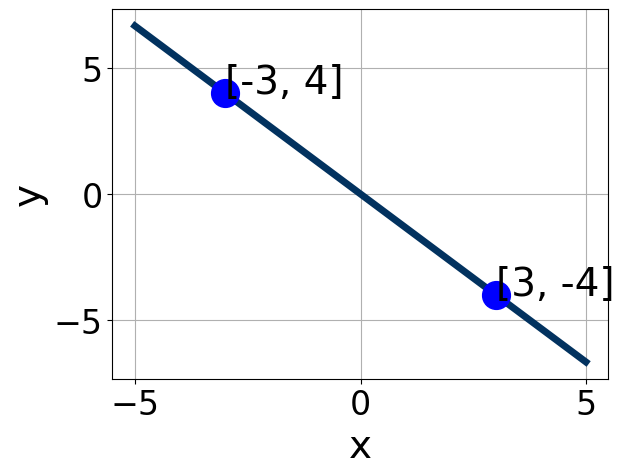
\includegraphics[width=0.5\textwidth]{../Figures/linearGraphToStandardCopyC.png}
\end{center}
\begin{enumerate}[label=\Alph*.]
\item \( A \in [0.33, 2.33], \hspace{3mm} B \in [-1.2, 0.9], \text{ and } \hspace{3mm} C \in [-3, 6] \)
\item \( A \in [0.33, 2.33], \hspace{3mm} B \in [0.2, 2.1], \text{ and } \hspace{3mm} C \in [-3, 6] \)
\item \( A \in [3, 5], \hspace{3mm} B \in [2.9, 4.9], \text{ and } \hspace{3mm} C \in [-3, 6] \)
\item \( A \in [3, 5], \hspace{3mm} B \in [-4.6, -2.1], \text{ and } \hspace{3mm} C \in [-3, 6] \)
\item \( A \in [-5, -1], \hspace{3mm} B \in [-4.6, -2.1], \text{ and } \hspace{3mm} C \in [-3, 6] \)

\end{enumerate} }
\litem{
Find the equation of the line described below. Write the linear equation in the form $ y=mx+b $ and choose the intervals that contain $m$ and $b$.\[ \text{Parallel to } 5 x + 6 y = 12 \text{ and passing through the point } (9, 2). \]\begin{enumerate}[label=\Alph*.]
\item \( m \in [-1.23, -0.94] \hspace*{3mm} b \in [6.2, 11.4] \)
\item \( m \in [-0.98, -0.67] \hspace*{3mm} b \in [-10.7, -8.1] \)
\item \( m \in [-0.98, -0.67] \hspace*{3mm} b \in [6.2, 11.4] \)
\item \( m \in [0.59, 0.84] \hspace*{3mm} b \in [-6.6, -2.7] \)
\item \( m \in [-0.98, -0.67] \hspace*{3mm} b \in [-7.4, -6.1] \)

\end{enumerate} }
\litem{
Solve the equation below. Then, choose the interval that contains the solution.\[ -7(-11x + 8) = -9(-5x -4) \]\begin{enumerate}[label=\Alph*.]
\item \( x \in [-0.79, -0.5] \)
\item \( x \in [0.45, 0.7] \)
\item \( x \in [2.28, 3.02] \)
\item \( x \in [-0.02, 0.34] \)
\item \( \text{There are no real solutions.} \)

\end{enumerate} }
\litem{
Find the equation of the line described below. Write the linear equation in the form $ y=mx+b $ and choose the intervals that contain $m$ and $b$.\[ \text{Perpendicular to } 7 x - 4 y = 12 \text{ and passing through the point } (-8, -10). \]\begin{enumerate}[label=\Alph*.]
\item \( m \in [-0.8, -0.5] \hspace*{3mm} b \in [14.57, 15.57] \)
\item \( m \in [-0.8, -0.5] \hspace*{3mm} b \in [-4, 0] \)
\item \( m \in [-2.2, -1.59] \hspace*{3mm} b \in [-15.57, -10.57] \)
\item \( m \in [-0.8, -0.5] \hspace*{3mm} b \in [-15.57, -10.57] \)
\item \( m \in [0.38, 1.39] \hspace*{3mm} b \in [-8.43, -4.43] \)

\end{enumerate} }
\litem{
Solve the linear equation below. Then, choose the interval that contains the solution.\[ \frac{9x -8}{7} - \frac{9x + 5}{3} = \frac{-9x -7}{4} \]\begin{enumerate}[label=\Alph*.]
\item \( x \in [-4.3, -3.1] \)
\item \( x \in [9.5, 12.2] \)
\item \( x \in [-0.6, 0.4] \)
\item \( x \in [1.2, 3] \)
\item \( \text{There are no real solutions.} \)

\end{enumerate} }
\litem{
First, find the equation of the line containing the two points below. Then, write the equation in the form $ y=mx+b $ and choose the intervals that contain $m$ and $b$.\[ (-10, 10) \text{ and } (-8, -4) \]\begin{enumerate}[label=\Alph*.]
\item \( m \in [-7, 0] \hspace*{3mm} b \in [15, 26] \)
\item \( m \in [2, 13] \hspace*{3mm} b \in [49, 59] \)
\item \( m \in [-7, 0] \hspace*{3mm} b \in [2, 6] \)
\item \( m \in [-7, 0] \hspace*{3mm} b \in [-64, -56] \)
\item \( m \in [-7, 0] \hspace*{3mm} b \in [57, 66] \)

\end{enumerate} }
\litem{
Write the equation of the line in the graph below in Standard Form $Ax+By=C$. Then, choose the intervals that contain $A, B, \text{ and } C$.
\begin{center}
    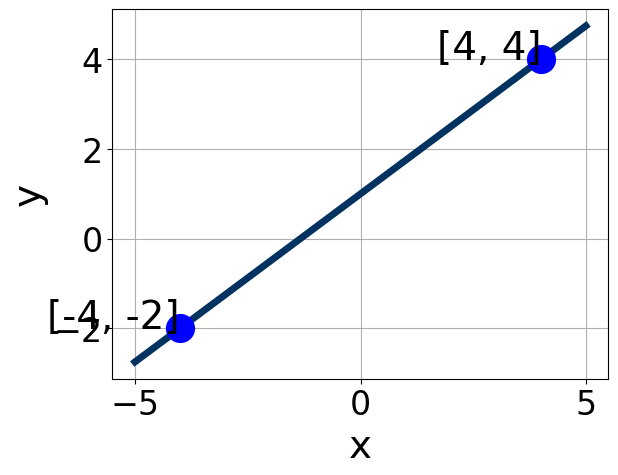
\includegraphics[width=0.5\textwidth]{../Figures/linearGraphToStandardC.png}
\end{center}
\begin{enumerate}[label=\Alph*.]
\item \( A \in [2.6, 5.1], \hspace{3mm} B \in [-4.19, -2.6], \text{ and } \hspace{3mm} C \in [-5.2, -2.9] \)
\item \( A \in [-2.4, 2.1], \hspace{3mm} B \in [-1.84, -0.71], \text{ and } \hspace{3mm} C \in [-1.1, 0.7] \)
\item \( A \in [2.6, 5.1], \hspace{3mm} B \in [2.4, 4.21], \text{ and } \hspace{3mm} C \in [2.8, 4.9] \)
\item \( A \in [-2.4, 2.1], \hspace{3mm} B \in [0.92, 1.29], \text{ and } \hspace{3mm} C \in [0.7, 1.2] \)
\item \( A \in [-3.2, -1.6], \hspace{3mm} B \in [2.4, 4.21], \text{ and } \hspace{3mm} C \in [2.8, 4.9] \)

\end{enumerate} }
\litem{
First, find the equation of the line containing the two points below. Then, write the equation in the form $ y=mx+b $ and choose the intervals that contain $m$ and $b$.\[ (-9, 11) \text{ and } (-2, -10) \]\begin{enumerate}[label=\Alph*.]
\item \( m \in [-5, 0] \hspace*{3mm} b \in [-24, -13] \)
\item \( m \in [-5, 0] \hspace*{3mm} b \in [-8, -7] \)
\item \( m \in [-5, 0] \hspace*{3mm} b \in [14, 17] \)
\item \( m \in [1, 5] \hspace*{3mm} b \in [-6, -3] \)
\item \( m \in [-5, 0] \hspace*{3mm} b \in [20, 24] \)

\end{enumerate} }
\litem{
Solve the equation below. Then, choose the interval that contains the solution.\[ -10(-5x -3) = -8(-9x -12) \]\begin{enumerate}[label=\Alph*.]
\item \( x \in [-7.5, -4.6] \)
\item \( x \in [-1.2, -0.3] \)
\item \( x \in [5, 6.7] \)
\item \( x \in [-4.3, -2.1] \)
\item \( \text{There are no real solutions.} \)

\end{enumerate} }
\end{enumerate}

\end{document}